\documentclass[11pt]{charter}

% El títulos de la memoria, se usa en la carátula y se puede usar el cualquier lugar del documento con el comando \ttitle
\titulo{Punto de cobro sin contacto para uso temporal de equipos} 

% Nombre del posgrado, se usa en la carátula y se puede usar el cualquier lugar del documento con el comando \degreename
%\posgrado{Carrera de Especialización en Sistemas Embebidos} 
\posgrado{Carrera de Especialización en Internet de las Cosas} 
%\posgrado{Carrera de Especialización en Intelegencia Artificial}
%\posgrado{Maestría en Sistemas Embebidos} 
%\posgrado{Maestría en Internet de las cosas}

% Tu nombre, se puede usar el cualquier lugar del documento con el comando \authorname
\autor{Mariano Graziano} 

% El nombre del director y co-director, se puede usar el cualquier lugar del documento con el comando \supname y \cosupname y \pertesupname y \pertecosupname
\director{Santiago Salamandri}
\pertenenciaDirector{UBA - UNC} 
% FIXME:NO IMPLEMENTADO EL CODIRECTOR ni su pertenencia
\codirector{} % si queda vacio no se deberíá incluir 
\pertenenciaCoDirector{}

% Nombre del cliente, quien va a aprobar los resultados del proyecto, se puede usar con el comando \clientename y \empclientename
\cliente{Fernando Abramowicz}
\empresaCliente{Cliente}

% Nombre y pertenencia de los jurados, se pueden usar el cualquier lugar del documento con el comando \jurunoname, \jurdosname y \jurtresname y \perteunoname, \pertedosname y \pertetresname.
\juradoUno{Nombre y Apellido (1)}
\pertenenciaJurUno{pertenencia (1)} 
\juradoDos{Nombre y Apellido (2)}
\pertenenciaJurDos{pertenencia (2)}
\juradoTres{Nombre y Apellido (3)}
\pertenenciaJurTres{pertenencia (3)}
 
\fechaINICIO{25 de Agosto de 2020}		%Fecha de inicio de la cursada de GdP \fechaInicioName
\fechaFINALPlanificacion{13 de Octubre de 2020} 	%Fecha de final de cursada de GdP
\fechaFINALTrabajo{1 de Septiembre de 2021}		%Fecha de defensa pública del trabajo final


\begin{document}

\maketitle
\thispagestyle{empty}
\pagebreak


\thispagestyle{empty}
{\setlength{\parskip}{0pt}
\tableofcontents{}
}
\pagebreak


\section{Registros de cambios}
\label{sec:registro}


\begin{table}[ht]
\label{tab:registro}
\centering
\begin{tabularx}{\linewidth}{@{}|c|X|c|@{}}
\hline
\rowcolor[HTML]{C0C0C0} 
Revisión & \multicolumn{1}{c|}{\cellcolor[HTML]{C0C0C0}Detalles de los cambios realizados} & Fecha      \\ \hline
1.0      & Creación del documento y redacción de puntos 1,2,3,4 y 6  & 06/09/2020 \\ \hline
1.1      & Corrección de observaciones recibidas y adhesión de historias de usuarios                                                                 & 15/09/2020 \\ \hline
1.2      & Puntos 6-17 pendientes. &05/10/2020 \\ \hline
1.3      & Correción a observaciones recibidas. &12/10/2020 \\ \hline
%		   Con texto partido \newline
%		   En varias líneas \newline
%		   A propósito                                                     %& dd/mm/aaaa \\ \hline
\end{tabularx}
\end{table}

\pagebreak



\section{Acta de constitución del proyecto}
\label{sec:acta}

\begin{flushright}
Buenos Aires, \fechaInicioName
\end{flushright}

\vspace{2cm}

Por medio de la presente se acuerda con el Ing. \authorname\hspace{1px} que su Trabajo Final de la \degreename\hspace{1px} se titulará ``\ttitle'', consistirá esencialmente en el diseño y creación de un dispositivo que valide la identidad de un usuario y se integre con distintos medios de pagos para hacer uso de equipos electrónicos por lapsos predefinidos de tiempo, y tendrá un presupuesto preliminar estimado de 642 hs de trabajo y \$ 871.250, con fecha de inicio \fechaInicioName\hspace{1px} y fecha de presentación pública \fechaFinalName.

Se adjunta a esta acta la planificación inicial.

\vfill

% Esta parte se construye sola con la información que hayan cargado en el preámbulo del documento y no debe modificarla
\begin{table}[ht]
\centering
\begin{tabular}{ccc}
\begin{tabular}[c]{@{}c@{}}Ariel Lutenberg \\ Director posgrado FIUBA\end{tabular} & \hspace{2cm} & \begin{tabular}[c]{@{}c@{}}\clientename \\ \empclientename  \end{tabular} \vspace{2.5cm} \\ 
\multicolumn{3}{c}{\begin{tabular}[c]{@{}c@{}} \supname \\ Director del Trabajo Final\end{tabular}} \vspace{2.5cm} \\
%\begin{tabular}[c]{@{}c@{}}\jurunoname \\ Jurado del Trabajo Final\end{tabular}     &  & \begin{tabular}[c]{@{}c@{}}\jurdosname\\ Jurado del Trabajo Final\end{tabular}  \vspace{2.5cm}  \\
%\multicolumn{3}{c}{\begin{tabular}[c]{@{}c@{}} \jurtresname\\ Jurado del Trabajo Final\end{tabular}} \vspace{.5cm}                                                                     
\end{tabular}
\end{table}




\section{Descripción técnica-conceptual del proyecto a realizar}
\label{sec:descripcion}


En la actualidad distintos tipos de equipamiento de uso compartido como televisores en centros de salud, lavarropas en edificios o barrios cerrados o sistemas de iluminación en complejos deportivos,  entre otros, utilizan la modalidad de compra de fichas o monedas para habilitar el uso del equipo en cuestión por un tiempo determinado.


Las fichas se insertan en un dispositivo-temporizador que reconoce el valor de las mismas y al cubrir un monto preestablecido habilita el uso del equipamiento por un tiempo determinado. 

Este equipamiento se administra de manera desatendida lo cual tiene las siguientes: 

\begin{itemize}
\item Cada uno de los dispositivos debe configurarse de modo presencial y periódicamente debe vaciarse el cofre de recaudación.

\item No hay forma remota de saber si el electrodoméstico esta siendo usado por otro vecino.
\item Las fichas deben adquirirse en los kioskos de cercanía, que suelen desabastecerse casi inmediatamente en cuanto el proveedor las suministra.
\end{itemize}


El presente proyecto expresa el desafío de compatibilizar y articular todos los contenidos curriculares de la especialización con servicios de pago disponibles en el país con el fin de crear un dispositivo que permita al usuario de lavarropas comunitarios tener distintas alternativas digitales al pagar y no depender de la disponibilidad de cospeles en un comercio de cercanía. 
 

Una de las principales motivaciones para llevar adelante este proyecto se produce en el contexto de la pandemia de SARS-COV-2. El aislamiento social y preventivo que está requiere, pone de manifiesto la obsolescencia de la practica actual en algo tan esencial como el lavado de ropa, de ir hasta comercios específicos y manipular dinero en efectivo.  

Como se puede ver en la Fig. 2, se reemplaza la utilización de fichas y toda la logística que esto implica por una aplicación móvil o un medio RFID.

El usuario del equipo podrá cargarle saldo por un medio de pago online (gateway de pago o transferencia PEI) u offline (corresponsalías extrabancarias como Rapipago o Pago Fácil).

El dispositivo estará instalado próximo al equipo a utilizar y administrará el uso de la energía eléctrica del equipo.

Al querer utilizar el equipamiento, el usuario acerca su medio de pago al dispositivo el cual validará contra un servicio remoto que el medio de pago tenga saldo y el costo y plazo definido para ese dispositivo.

Se inicia una cuenta regresiva por el plazo contratado en la pantalla del dispositivo y la misma se replica en la aplicación multiplataforma del usuario. El dispositivo contará con un teclado numérico como interface de troubleshooting o uso alternativo a la tarjeta. 

Como complemento al desarrollo del dispositivo la innovación en este proyecto pasará por investigar la factibilidad técnica y económica de implementar en un proyecto de este tipo la tecnología distribuida y potencial protocolo IOTA como medio de intercambio de información entre los distintos dispositivos intervinientes.
\vspace{25px}
\begin{figure}[htpb]
\centering 
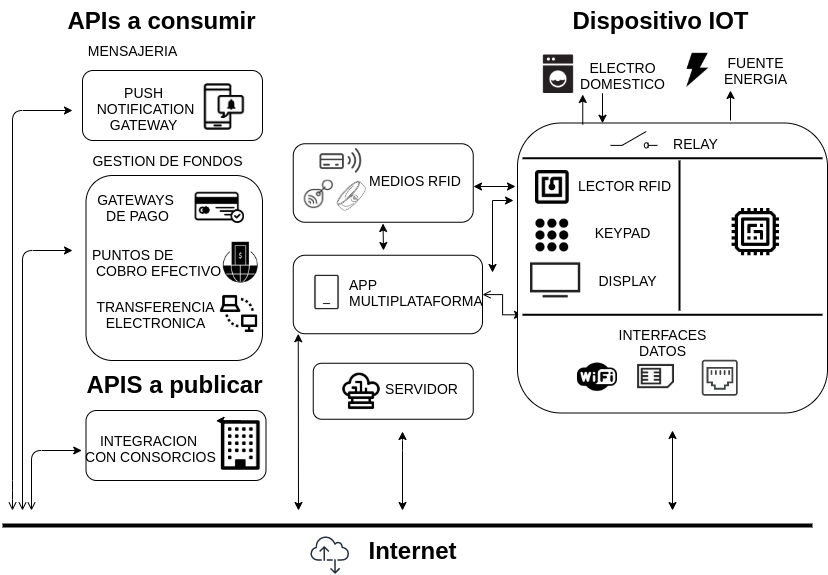
\includegraphics[width=.7\textwidth]{./Figuras/diagBloques.png}
\caption{Diagrama en bloques del sistema}
\label{fig:diagBloques}
\end{figure}
\vspace{25px}


\newpage 
\newpage 

\section{Identificación y análisis de los interesados}
\label{sec:interesados}

\begin{table}[ht]
\caption{Identificación de los interesados}
\label{tab:interesados}
\begin{tabularx}{\linewidth}{@{}|l|X|X|l|@{}}
\hline
\rowcolor[HTML]{C0C0C0} 
Rol           & Nombre y Apellido & Organización 	& Puesto 	\\ \hline
Cliente   &\clientename   &           -   	&     -   	\\ \hline
Responsable   & \authorname       & FIUBA        	& Alumno 	\\ \hline
Orientador    & \supname	      & \pertesupname 	& Director	Trabajo final \\ \hline
Consulta     & Alfonso Alvarez	      & -  	& - \\ \hline
%Equipo        & miembro1 \newline 
%				miembro2          &              	&        	\\ \hline
Opositores    & Empresas que provean servicios de laundrys.                   &              -	&       - 	\\ \hline
Usuario final & Habitantes de complejos con área de lavarropas compartido & -             	&     -   	\\ \hline
\end{tabularx}
\end{table}

Dado que se trata de un emprendimiento personal, los roles del cliente y consultor son voluntarios elegidos por su capacidad de aportar valor en temas comerciales y técnicos respectivamente al proyecto.
 
\newpage 

\section{1. Propósito del proyecto}
\label{sec:proposito}

 Este proyecto tiene tres propósitos: 
 
 \begin{itemize}
\item El principal es digitalizar el proceso de pago en servicios que aun utilizan fichas o monedas.
\item En segundo lugar adquirir los conocimientos propios del ciclo de vida de un proyecto de IOT con servicios basados en la nube e integración y desarrollo de con APIs desde su planificación hasta su ejecución.
\item Por último documentar en un contexto académico el análisis y potencial de la tecnología distribuida IOTA.

\end{itemize}
 
  

\section{2. Alcance del proyecto}
\label{sec:alcance}

El presente proyecto incluye: 
\begin{itemize}
		\item Diseño y armado de un dispositivo de cobro sin contacto.  
		\item Diseño y desarrollo de aplicación multiplataforma tanto para usuarios como para administradores del sistema. 
		\item Diseño de API para disponibilizar el acceso a terceros.
		\item Investigación sobre tecnología IOTA y su impacto un proyecto de este estilo.
\end{itemize}		
 El presente proyecto no incluye:
\begin{itemize}	
		\item La integración con Plataformas de administradores de consorcios.
		\item La integración con entornos productivos de gateways de pago o banca online. 		
\end{itemize}		 
\section{3. Supuestos del proyecto}
\label{sec:supuestos}
Para el desarrollo del presente proyecto se supone que:
\begin{itemize}
\item Se podrá acceder a entornos sandbox de gateways de pago y banca online.
\item Todo el hardware necesario podrá adquirirse en el país.
\item Dentro de los contenidos curriculares de la carrera es factible que se incluyan contenidos que permitan cubrir algunos de los requerimientos de manera mas eficiente a la propuesta en este documento. Los mismos se aplicarán en tanto el beneficio lo amerite y se pueda implementar la  mejora dentro de los plazos estipulados en el Acta de Constitución.
\end{itemize}

\section{4. Requerimientos}
\label{sec:requerimientos}

\begin{enumerate}
\item Requerimientos funcionales del dispositivo:
	\begin{enumerate}
\item El punto de cobro debe estar conectado por uno o más medios a  Internet de manera estable.
\item El usuario debe poder identificarse  con un medio RFID o su teléfono celular sin tener contacto físico con el dispositivo y con la menor interacción posible.
\item En caso de corte de suministro eléctrico debe poder reiniciarse y volver al estado inmediato anterior al corte.
\item Deberá mostrar en la pantalla el estado del dispositivo y en caso de estar ocupado el tiempo restante.
\item Deberá contar con un teclado numérico como alternativa para usuarios que no quieran utilizar un medio electrónico de contacto y/o como interfaz de control en el sitio asumiendo que es la única manera de tomar control del dispositivo.
\end{enumerate}
\item Requerimientos funcionales de la aplicación multiplataforma para el administrador:
	\begin{enumerate} 
\item Deberá poder gestionar la creación de nodos y la asignación de dispositivos a cada nodo. 
\item Deberá poder asignar usuarios administradores a cada uno de los nodos.
\item Deberá poder gestionar el costo y plazo de los lavarropas que están conectados a lavarropas.
\item Deberá poder gestionar el alta masiva y la forma de validación de los usuarios del nodo.
\item Deberá poder definir descuentos / promociones en función del nivel de usuario.
\item Deberá contar con un dashboard con el estado y niveles de uso de cada uno de los dispositivos. 
\item Deberá poder definir los medios de cobro y de pago asociados al nodo. 
	\end{enumerate}
\item Requerimientos funcionales de la aplicación multiplataforma para el usuario final: 
\begin{enumerate} 
\item Deberá poder cargar saldo a su cuenta con los medios de pagos habilitados.
\item Deberá poder gestionar los medios RFID asociados a su cuenta. 
\item Deberá poder ver la disponibilidad de los equipos a los que tiene acceso. 
	\end{enumerate}
\item Requerimientos no funcionales.
\begin{enumerate}
\item Se debe loguear toda la información relevante a los fines de diagnosticar posibles problemas y/o mejoras al sistema.
\item Toda la información sensible del usuario debe almacenarse y transferirse de manera segura acorde a los estándares de seguridad de la industria. 
	\end{enumerate}
\end{enumerate}

\section{Historias de usuarios (\textit{Product backlog})}
\label{sec:backlog}


A continuación se listan las historias de usuario identificadas para el proyecto. Se agrega una ponderación (columna "Pond.") que describe el nivel del esfuerzo que se estima tenga la historia y una Prioridad (columna "Pri.") que hace referencia a la prioridad de 1 a 5, siendo 5 lo mas prioritario.

\begin{table}[]
\resizebox{\textwidth}{!}{%
\begin{tabular}{lllllc}
\hline
\rowcolor[HTML]{FFFC9E} 
Nro                      & " .. Como... "                           & "... quiero ..."                                                                                                                                                          & "... para que pueda ..."                                                                                                                       & Pond.                      & Pri.                   \\ \hline
\multicolumn{1}{|l|}{1}  & \multicolumn{1}{l|}{Usuario}    & \multicolumn{1}{l|}{Saber como funciona el servicio}                                                                                                                & \multicolumn{1}{l|}{\begin{tabular}[c]{@{}l@{}}Entender que tengo que hacer para \\ usar el servicio.\end{tabular}}                      & \multicolumn{1}{l|}{Baja}  & \multicolumn{1}{c|}{3} \\ \hline
\multicolumn{1}{|l|}{2}  & \multicolumn{1}{l|}{Usuario}    & \multicolumn{1}{l|}{Darme de alta en el servicio.}                                                                                                                  & \multicolumn{1}{l|}{Comprar créditos para utilizar el servicio.}                                                                         & \multicolumn{1}{l|}{Media} & \multicolumn{1}{c|}{5} \\ \hline
\multicolumn{1}{|l|}{3}  & \multicolumn{1}{l|}{Usuario}    & \multicolumn{1}{l|}{\begin{tabular}[c]{@{}l@{}}Comprar créditos por medio de tarjeta de \\ crédito / tarjeta de débito / \\ efectivo o transferencia.\end{tabular}} & \multicolumn{1}{l|}{Utilizar el servicio.}                                                                                               & \multicolumn{1}{l|}{Alta}  & \multicolumn{1}{c|}{5} \\ \hline
\multicolumn{1}{|l|}{4}  & \multicolumn{1}{l|}{Usuario}    & \multicolumn{1}{l|}{\begin{tabular}[c]{@{}l@{}}Que el costo del lavado \\ se acredite en las expensas.\end{tabular}}                                                & \multicolumn{1}{l|}{\begin{tabular}[c]{@{}l@{}}No tener que andar preocupándome\\ por cargar saldo previamente.\end{tabular}}            & \multicolumn{1}{l|}{Alta}  & \multicolumn{1}{c|}{3} \\ \hline
\multicolumn{1}{|l|}{5}  & \multicolumn{1}{l|}{Usuario}    & \multicolumn{1}{l|}{Pagar el servicio con un teléfono Android.}                                                                                                     & \multicolumn{1}{l|}{Utilizar el servicio.}                                                                                               & \multicolumn{1}{l|}{Alta}  & \multicolumn{1}{c|}{5} \\ \hline
\multicolumn{1}{|l|}{6}  & \multicolumn{1}{l|}{Usuario}    & \multicolumn{1}{l|}{Pagar el servicio con un teléfono IOS.}                                                                                                         & \multicolumn{1}{l|}{Utilizar el servicio.}                                                                                               & \multicolumn{1}{l|}{Alta}  & \multicolumn{1}{c|}{3} \\ \hline
\multicolumn{1}{|l|}{7}  & \multicolumn{1}{l|}{Usuario}    & \multicolumn{1}{l|}{Pagar el servicio con una tarjeta RFID.}                                                                                                        & \multicolumn{1}{l|}{\begin{tabular}[c]{@{}l@{}}Utilizar el servicio sin tener\\ que usar el teléfono,\end{tabular}}                      & \multicolumn{1}{l|}{Alta}  & \multicolumn{1}{c|}{5} \\ \hline
\multicolumn{1}{|l|}{10} & \multicolumn{1}{l|}{Usuario}    & \multicolumn{1}{l|}{\begin{tabular}[c]{@{}l@{}}Des asociar medio RFID / teléfono \\ celular por extravío\end{tabular}}                                              & \multicolumn{1}{l|}{Resguardar el saldo en caso de perdida.}                                                                             & \multicolumn{1}{l|}{Media} & \multicolumn{1}{c|}{3} \\ \hline
\multicolumn{1}{|l|}{11} & \multicolumn{1}{l|}{Usuario}    & \multicolumn{1}{l|}{\begin{tabular}[c]{@{}l@{}}Poder usar el servicio si el sistema \\ ante un problema de la terminal.\end{tabular}}                               & \multicolumn{1}{l|}{\begin{tabular}[c]{@{}l@{}}No resultar damnificado por un \\ problema ajeno a mi.\end{tabular}}                      & \multicolumn{1}{l|}{Media} & \multicolumn{1}{c|}{4} \\ \hline
\multicolumn{1}{|l|}{12} & \multicolumn{1}{l|}{Usuario}    & \multicolumn{1}{l|}{\begin{tabular}[c]{@{}l@{}}Saber cuanto tiempo falta para que \\ se libere algún equipo del nodo\end{tabular}}                                  & \multicolumn{1}{l|}{No ir hasta el nodo innecesariamente.}                                                                               & \multicolumn{1}{l|}{Baja}  & \multicolumn{1}{c|}{3} \\ \hline
\multicolumn{1}{|l|}{13} & \multicolumn{1}{l|}{Usuario}    & \multicolumn{1}{l|}{\begin{tabular}[c]{@{}l@{}}Saber cuanto tiempo falta para que\\  termine el servicio contratado\end{tabular}}                                   & \multicolumn{1}{l|}{\begin{tabular}[c]{@{}l@{}}Saber si puedo ir a retirar la ropa sin tener\\  que ir hasta el lugar.\end{tabular}}     & \multicolumn{1}{l|}{Baja}  & \multicolumn{1}{c|}{5} \\ \hline
\multicolumn{1}{|l|}{14} & \multicolumn{1}{l|}{Usuario}    & \multicolumn{1}{l|}{\begin{tabular}[c]{@{}l@{}}Poder gestionar las notificaciones \\ del sistema.\end{tabular}}                                                     & \multicolumn{1}{l|}{Recibir las notificaciones que quiero.}                                                                              & \multicolumn{1}{l|}{Media} & \multicolumn{1}{c|}{3} \\ \hline
\multicolumn{1}{|l|}{15} & \multicolumn{1}{l|}{Usuario}    & \multicolumn{1}{l|}{Ver estadísticas de uso de mi cuenta}                                                                                                           & \multicolumn{1}{l|}{Saber mi historial de uso y cargas}                                                                                  & \multicolumn{1}{l|}{Media} & \multicolumn{1}{c|}{3} \\ \hline
\multicolumn{1}{|l|}{16} & \multicolumn{1}{l|}{Usuario}    & \multicolumn{1}{l|}{\begin{tabular}[c]{@{}l@{}}Descargar el comprobante\\  de crédito comprado\end{tabular}}                                                        & \multicolumn{1}{l|}{Tener la factura del gasto realizado}                                                                                & \multicolumn{1}{l|}{Alta}  & \multicolumn{1}{c|}{4} \\ \hline
\multicolumn{1}{|l|}{17} & \multicolumn{1}{l|}{Usuario}    & \multicolumn{1}{l|}{\begin{tabular}[c]{@{}l@{}}Recomendar a potenciales \\ usuarios / nodos.\end{tabular}}                                                          & \multicolumn{1}{l|}{Recibir beneficios por la recomendación.}                                                                            & \multicolumn{1}{l|}{Baja}  & \multicolumn{1}{c|}{2} \\ \hline
\multicolumn{1}{|l|}{18} & \multicolumn{1}{l|}{Usuario}    & \multicolumn{1}{l|}{\begin{tabular}[c]{@{}l@{}}Quiero devolver crédito \\ comprado por error.\end{tabular}}                                                         & \multicolumn{1}{l|}{Recuperar dinero.}                                                                                                   & \multicolumn{1}{l|}{Media} & \multicolumn{1}{c|}{4} \\ \hline
\multicolumn{1}{|l|}{19} & \multicolumn{1}{l|}{Usuario}    & \multicolumn{1}{l|}{\begin{tabular}[c]{@{}l@{}}Cambiar contraseña y datos \\ personales de aplicación\end{tabular}}                                                 & \multicolumn{1}{l|}{Administrar la seguridad de su cuenta}                                                                               & \multicolumn{1}{l|}{Baja}  & \multicolumn{1}{c|}{4} \\ \hline
\multicolumn{1}{|l|}{20} & \multicolumn{1}{l|}{Operador}   & \multicolumn{1}{l|}{\begin{tabular}[c]{@{}l@{}}Gestionar altas y bajas de nodos y \\ dispositivos en cada nodo.\end{tabular}}                                       & \multicolumn{1}{l|}{Asignar equipos a un edificio.}                                                                                      & \multicolumn{1}{l|}{Media} & \multicolumn{1}{c|}{3} \\ \hline
\multicolumn{1}{|l|}{21} & \multicolumn{1}{l|}{Operador}   & \multicolumn{1}{l|}{\begin{tabular}[c]{@{}l@{}}Monitorear logs de los puntos \\ de cobro en un nodo.\end{tabular}}                                                  & \multicolumn{1}{l|}{\begin{tabular}[c]{@{}l@{}}Verificar el correcto \\ funcionamiento del dispositivo\end{tabular}}                     & \multicolumn{1}{l|}{Alta}  & \multicolumn{1}{c|}{4} \\ \hline
\multicolumn{1}{|l|}{22} & \multicolumn{1}{l|}{Operador}   & \multicolumn{1}{l|}{\begin{tabular}[c]{@{}l@{}}Monitorear conectividad de los puntos\\ de cada nodo.\end{tabular}}                                                  & \multicolumn{1}{l|}{\begin{tabular}[c]{@{}l@{}}Verificar el correcto\\ funcionamiento del dispositivo\end{tabular}}                      & \multicolumn{1}{l|}{Alta}  & \multicolumn{1}{c|}{3} \\ \hline
\multicolumn{1}{|l|}{23} & \multicolumn{1}{l|}{Operador}   & \multicolumn{1}{l|}{Parametrizar de Alertas y Notificaciones.}                                                                                                      & \multicolumn{1}{l|}{\begin{tabular}[c]{@{}l@{}}Tomar conocimiento \\ de eventos a priorizar.\end{tabular}}                               & \multicolumn{1}{l|}{Media} & \multicolumn{1}{c|}{4} \\ \hline
\multicolumn{1}{|l|}{24} & \multicolumn{1}{l|}{Comerc.}    & \multicolumn{1}{l|}{Definir política de precios – descuentos.}                                                                                                      & \multicolumn{1}{l|}{\begin{tabular}[c]{@{}l@{}}Incentivar el uso de uno \\ u otro medio de pago.\end{tabular}}                           & \multicolumn{1}{l|}{Alta}  & \multicolumn{1}{c|}{3} \\ \hline
\multicolumn{1}{|l|}{25} & \multicolumn{1}{l|}{Comerc.}    & \multicolumn{1}{l|}{\begin{tabular}[c]{@{}l@{}}Visualizar cantidad de ventas \\ por dispositivo y/o nodo.\end{tabular}}                                             & \multicolumn{1}{l|}{\begin{tabular}[c]{@{}l@{}}Hacer seguimiento \\ de ventas y rentabilidad\end{tabular}}                               & \multicolumn{1}{l|}{Alta}  & \multicolumn{1}{c|}{3} \\ \hline
\multicolumn{1}{|l|}{26} & \multicolumn{1}{l|}{Finanzas}   & \multicolumn{1}{l|}{\begin{tabular}[c]{@{}l@{}}Verificar saldo circulante en \\ cuentas de usuarios.\end{tabular}}                                                  & \multicolumn{1}{l|}{\begin{tabular}[c]{@{}l@{}}Comparar contra el \\ existente en cuentas virtuales\end{tabular}}                        & \multicolumn{1}{l|}{Baja}  & \multicolumn{1}{c|}{3} \\ \hline
\multicolumn{1}{|l|}{27} & \multicolumn{1}{l|}{Seg. Info.} & \multicolumn{1}{l|}{Dar de alta usuarios al sistema de gestion}                                                                                                     & \multicolumn{1}{l|}{\begin{tabular}[c]{@{}l@{}}Permitir que los usuarios \\ puedan acceder al sistema\end{tabular}}                      & \multicolumn{1}{l|}{Media} & \multicolumn{1}{c|}{5} \\ \hline
\multicolumn{1}{|l|}{29} & \multicolumn{1}{l|}{Seg. Info.} & \multicolumn{1}{l|}{Asignar roles a un usuario}                                                                                                                     & \multicolumn{1}{l|}{Separar funciones entre los usuarios.}                                                                               & \multicolumn{1}{l|}{Media} & \multicolumn{1}{c|}{5} \\ \hline
\multicolumn{1}{|l|}{30} & \multicolumn{1}{l|}{Seg. Info.} & \multicolumn{1}{l|}{\begin{tabular}[c]{@{}l@{}}Dar de alta medios RFID que se pueden \\ usar en la plataforma.\end{tabular}}                                        & \multicolumn{1}{l|}{\begin{tabular}[c]{@{}l@{}}Que los usuarios puedan \\ dar de alta solo los medios habilitados.\end{tabular}}         & \multicolumn{1}{l|}{Baja}  & \multicolumn{1}{c|}{4} \\ \hline
\end{tabular}%
}
\end{table}

\section{5. Entregables principales del proyecto}
\label{sec:entregables}

\begin{itemize}
\item Prototipo funcional del dispositivo y de la aplicación a desarrollar.
\item Documento de conclusiones sobre viabilidad técnica / funcional de la implementación de una red IOTA  en este proyecto.
\item Diagrama esquemático del sistema.
\item Informe final
\end{itemize}


\section{6. Desglose del trabajo en tareas}
\label{sec:wbs}

\begin{enumerate}
\item Planificación y Análisis
	\begin{enumerate}
	\item Redacción de planificación del proyecto. (21 hs)
	\item Confección de presentación de planificación. (6 hs)
	\item Análisis y compra de componentes del dispositivo IOT. (18 hs)
	\item Análisis de viabilidad económica financiera. (6 hs)
	\item Análisis de protocolos de comunicación. (18 hs)
	\item Análisis APIs a consumir. (6 hs)
	\item Análisis de stack tecnológico a utilizar. (9 hs) 
	\item Análisis metodología de testing a utilizar (12 hs)
	\item Investigación sobre protocolo IOTA y su estado del arte. (12 hs) 
	\item Redacción de conclusiones de la etapa para desarrollo de informes.  (9 hs)
	\end{enumerate}	
\item Diseño del sistema
	\begin{enumerate}
	\item Diseño de base de datos. (9 hs)
	\item Diseño integración con servicios a consumir. (9 hs)
	\item Diseño de dispositivo IOT. (18 hs) 
	\item Diseño de aplicación multidispositivo. (18 hs)
	\item Diseño de pruebas de testing. (9 hs) 
\item Redacción de conclusiones de la etapa para desarrollo de informes.  (9 hs)
	\end{enumerate}
\item Desarrollo
	\begin{enumerate}
	\item Parametrización de contenedor según stack tecnológico. (6 hs)
	\item Construcción de dispositivo IOT. (18 hs) 
	\item Desarrollo de frontend usuarios.  (45 hs)
	\item Desarrollo de backend. (45  hs)
	\item Desarrollo de software en dispositivo IOT.  (45 hs)
	\item Integración con servicios en nube. (20 hs)
	\item Redacción de conclusiones de la etapa para desarrollo de memoria. (9 hs)
	\end{enumerate}
\item Testing y pruebas integrales.
	\begin{enumerate}
	\item Ejecución de pruebas de test. (30 hs)
	\item Documentación de pruebas de test. (20 hs)
	\item Redacción de conclusiones de la etapa para desarrollo de memoria. (9 hs)
	\end{enumerate}
\item Presentaciones
	\begin{enumerate}
	\item Elaboración de informes de avance. (21 hs)
	\item Elaboración de documento técnico y funcional de implementación de red IOTA en este proyecto. (18 hs)
	\item Elaboración de memoria de proyecto final. (120 hs) 
	\item Elaboración y preparación de presentación pública.  (15 hs)
	\end{enumerate}
\end{enumerate}

Cantidad total de horas: (642 h\textbf{s})


\section{7. Diagrama de Activity On Node}
\label{sec:AoN}



\begin{figure}[htpb]
\centering 
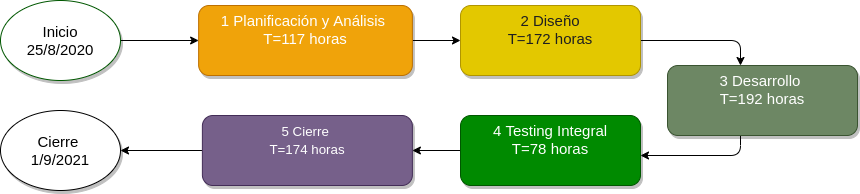
\includegraphics[width=.8\textwidth]{./Figuras/AoN.png}
\caption{Diagrama en \textit{Activity on Node}}
\label{fig:AoN}
\end{figure}




\section{8. Diagrama de Gantt}
\label{sec:gantt}

\begin{consigna}{red}
\begin{figure}[htpb]
\centering 
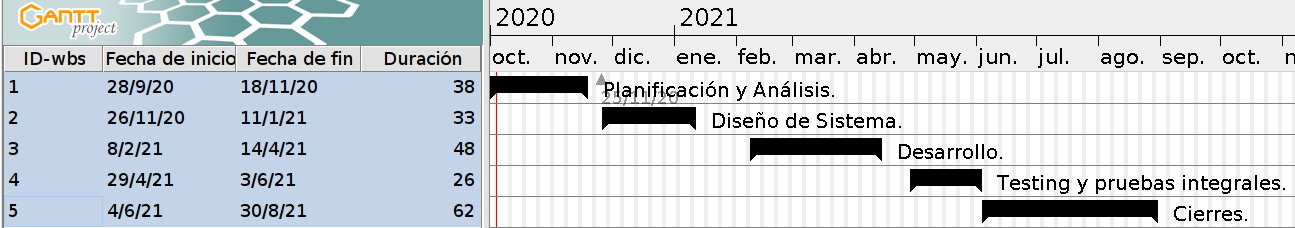
\includegraphics[width=.8\textwidth]{./Figuras/gantgeneral.png}
\caption{Diagrama de Gantt - Vista General}
\label{fig:GanttGeneral}
\end{figure}

\begin{figure}[htpb]
\centering 
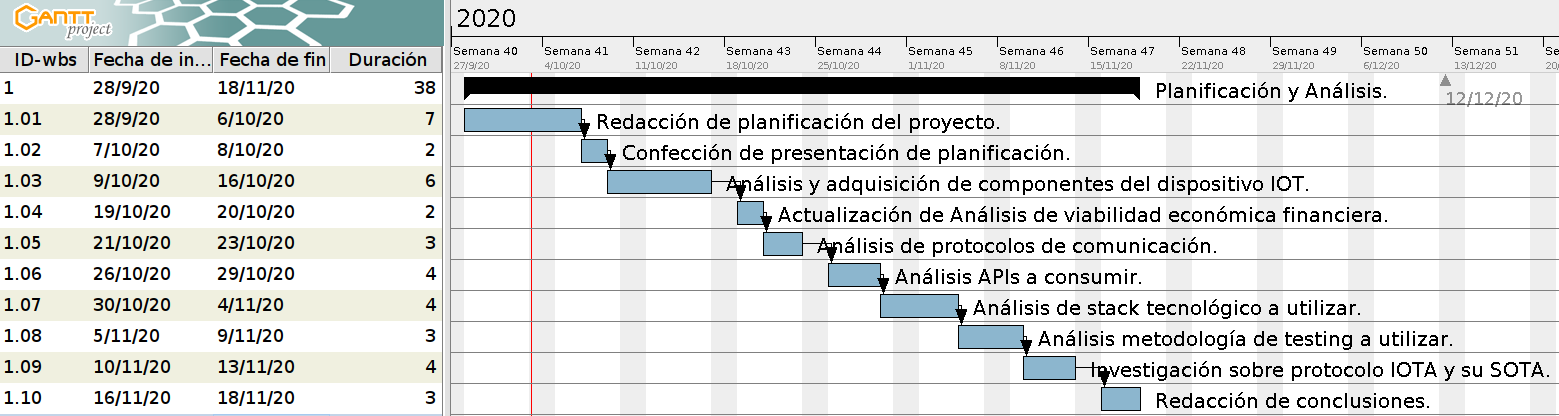
\includegraphics[width=.8\textwidth]{./Figuras/PlayAna.png}
\caption{Apertura de tareas - Etapa 1 - Planificación y Análisis}
\label{fig:GanttEtapa1}
\end{figure}

\begin{figure}[htpb]
\centering 
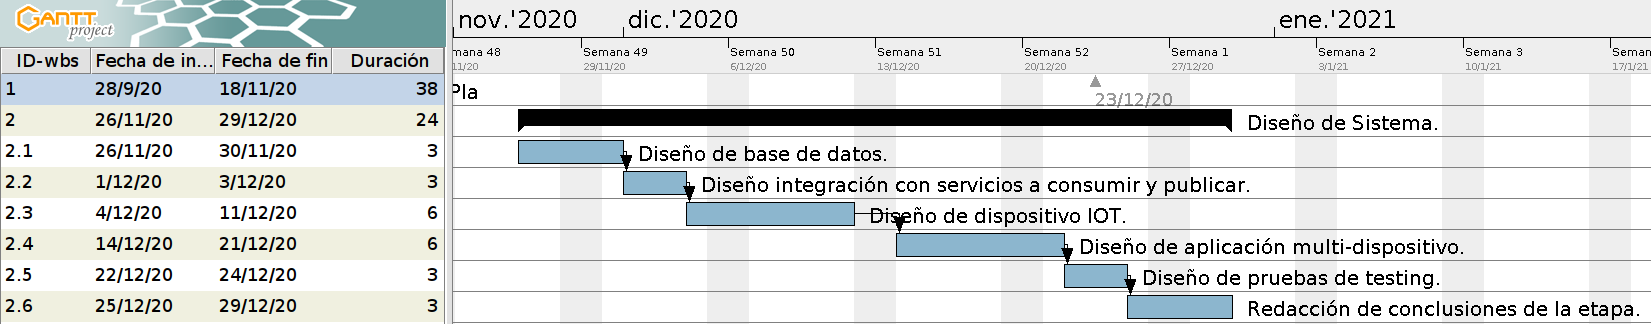
\includegraphics[width=.8\textwidth]{./Figuras/disenio.png}
\caption{Apertura de tareas - Etapa 2 - Diseño}
\label{fig:GanttEtapa2}
\end{figure}

\begin{figure}[htpb]
\centering 
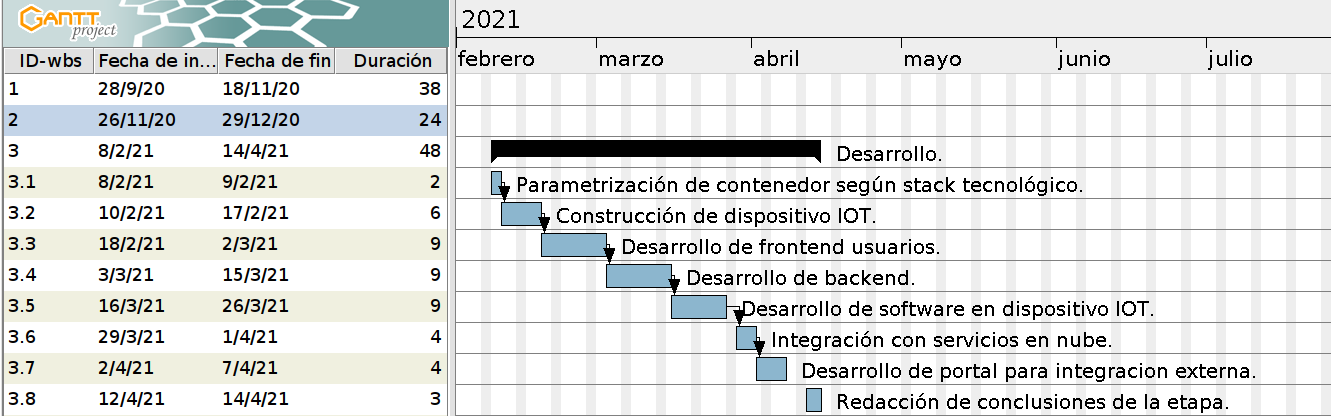
\includegraphics[width=.8\textwidth]{./Figuras/desarrollo.png}
\caption{Apertura de tareas - Etapa 3 - Desarrollo}
\label{fig:GanttEtapa4}
\end{figure}

\begin{figure}[htpb]
\centering 
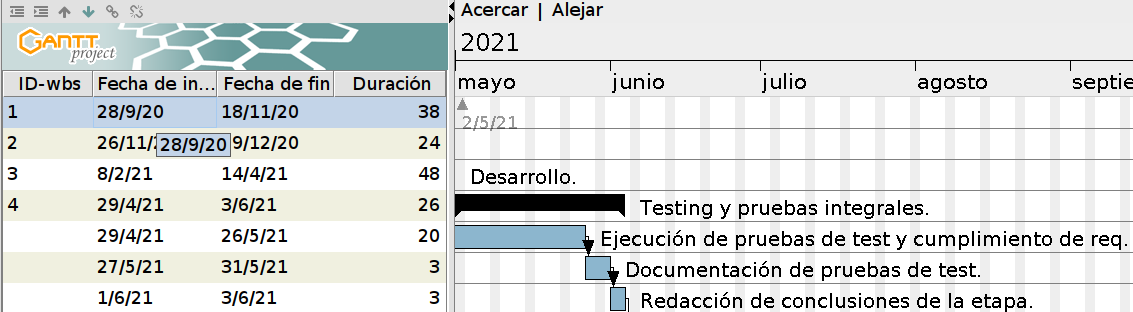
\includegraphics[width=.8\textwidth]{./Figuras/test.png}
\caption{Apertura de tareas - Etapa 5 - Test}
\label{fig:GanttEtapa5}
\end{figure}

\begin{figure}[htpb]
\centering 
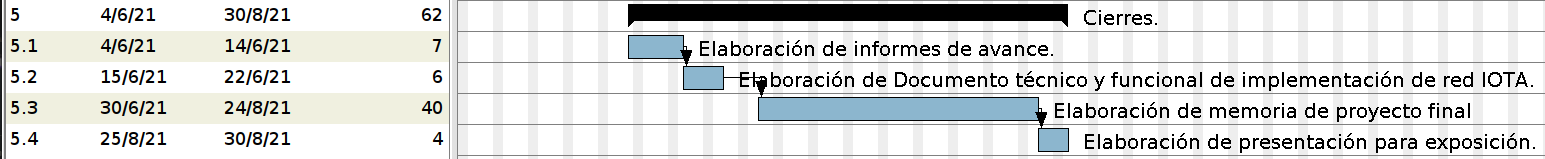
\includegraphics[width=.8\textwidth]{./Figuras/cierre.png}
\caption{Apertura de tareas - Etapa 6 - Cierre}
\label{fig:GanttEtapa6}
\end{figure}

\end{consigna}
\section{9. Matriz de uso de recursos de materiales}
\label{sec:recursos}

\begin{longtable}[c]{rlcccc}
\hline
\rowcolor[HTML]{C0C0C0} 
\multicolumn{1}{l}{\cellcolor[HTML]{C0C0C0}} & {\ul } & \multicolumn{4}{c}{\cellcolor[HTML]{C0C0C0}Recursos Requeridos} \\ \hline
\endfirsthead
%
\endhead
%
\rowcolor[HTML]{C0C0C0} 
\multicolumn{1}{|l|}{\cellcolor[HTML]{C0C0C0}WBS} & \multicolumn{1}{l|}{\cellcolor[HTML]{C0C0C0}Nombre de la Tarea} & \multicolumn{1}{c|}{\cellcolor[HTML]{C0C0C0}\begin{tabular}[c]{@{}c@{}}Puesto\\  de Trabajo\end{tabular}} & \multicolumn{1}{l|}{\cellcolor[HTML]{C0C0C0}\begin{tabular}[c]{@{}l@{}}Componen-\\ tes Electro-\\ nicos\\ (TBC)\end{tabular}} & \multicolumn{1}{l|}{\cellcolor[HTML]{C0C0C0}\begin{tabular}[c]{@{}l@{}}Medios\\  RFID\\ \\ (TBC)\end{tabular}} & \multicolumn{1}{l|}{\cellcolor[HTML]{C0C0C0}\begin{tabular}[c]{@{}l@{}}Herra-\\ mientas\\  (TBC)\end{tabular}} \\ \hline
\multicolumn{1}{|r|}{1.01} & \multicolumn{1}{l|}{Redacción de planificación del proyecto.} & \multicolumn{1}{c|}{21} & \multicolumn{1}{c|}{-} & \multicolumn{1}{c|}{-} & \multicolumn{1}{c|}{-} \\ \hline
\multicolumn{1}{|r|}{1.02} & \multicolumn{1}{l|}{Confección de presentación de planificación.} & \multicolumn{1}{c|}{6} & \multicolumn{1}{c|}{-} & \multicolumn{1}{c|}{-} & \multicolumn{1}{c|}{-} \\ \hline
\multicolumn{1}{|r|}{1.03} & \multicolumn{1}{l|}{\begin{tabular}[c]{@{}l@{}}Análisis y compra de componentes \\ del dispositivo IOT.\end{tabular}} & \multicolumn{1}{c|}{18} & \multicolumn{1}{c|}{-} & \multicolumn{1}{c|}{-} & \multicolumn{1}{c|}{-} \\ \hline
\multicolumn{1}{|r|}{1.04} & \multicolumn{1}{l|}{\begin{tabular}[c]{@{}l@{}}Actualización de análisis \\ de viabilidad económica financiera.\end{tabular}} & \multicolumn{1}{c|}{6} & \multicolumn{1}{c|}{-} & \multicolumn{1}{c|}{-} & \multicolumn{1}{c|}{-} \\ \hline
\multicolumn{1}{|r|}{1.05} & \multicolumn{1}{l|}{Análisis de protocolos de comunicación.} & \multicolumn{1}{c|}{18} & \multicolumn{1}{c|}{-} & \multicolumn{1}{c|}{-} & \multicolumn{1}{c|}{-} \\ \hline
\multicolumn{1}{|r|}{1.06} & \multicolumn{1}{l|}{Análisis APIs a consumir.} & \multicolumn{1}{c|}{6} & \multicolumn{1}{c|}{-} & \multicolumn{1}{c|}{-} & \multicolumn{1}{c|}{-} \\ \hline
\multicolumn{1}{|r|}{1.07} & \multicolumn{1}{l|}{Análisis de stack tecnológico a utilizar.} & \multicolumn{1}{c|}{9} & \multicolumn{1}{c|}{-} & \multicolumn{1}{c|}{-} & \multicolumn{1}{c|}{-} \\ \hline
\multicolumn{1}{|r|}{1.08} & \multicolumn{1}{l|}{Análisis metodología de testing a utilizar.} & \multicolumn{1}{c|}{12} & \multicolumn{1}{c|}{-} & \multicolumn{1}{c|}{-} & \multicolumn{1}{c|}{-} \\ \hline
\multicolumn{1}{|r|}{1.09} & \multicolumn{1}{l|}{\begin{tabular}[c]{@{}l@{}}Investigación sobre protocolo IOTA\\  y su estado del arte.\end{tabular}} & \multicolumn{1}{c|}{12} & \multicolumn{1}{c|}{-} & \multicolumn{1}{c|}{-} & \multicolumn{1}{c|}{-} \\ \hline
\multicolumn{1}{|r|}{1.10} & \multicolumn{1}{l|}{Redacción de conclusiones.} & \multicolumn{1}{c|}{9} & \multicolumn{1}{c|}{-} & \multicolumn{1}{c|}{-} & \multicolumn{1}{c|}{-} \\ \hline
\multicolumn{1}{|r|}{2.01} & \multicolumn{1}{l|}{Diseño de base de datos.} & \multicolumn{1}{c|}{9} & \multicolumn{1}{c|}{-} & \multicolumn{1}{c|}{-} & \multicolumn{1}{c|}{-} \\ \hline
\multicolumn{1}{|r|}{2.02} & \multicolumn{1}{l|}{\begin{tabular}[c]{@{}l@{}}Diseño integración \\ con servicios a consumir.\end{tabular}} & \multicolumn{1}{c|}{9} & \multicolumn{1}{c|}{-} & \multicolumn{1}{c|}{-} & \multicolumn{1}{c|}{} \\ \hline
\multicolumn{1}{|r|}{2.03} & \multicolumn{1}{l|}{Diseño de dispositivo IOT.} & \multicolumn{1}{c|}{18} & \multicolumn{1}{c|}{-} & \multicolumn{1}{c|}{-} & \multicolumn{1}{c|}{} \\ \hline
\multicolumn{1}{|r|}{2.04} & \multicolumn{1}{l|}{Diseño de aplicación multi-dispositivo.} & \multicolumn{1}{c|}{18} & \multicolumn{1}{c|}{-} & \multicolumn{1}{c|}{-} & \multicolumn{1}{c|}{} \\ \hline
\multicolumn{1}{|r|}{2.05} & \multicolumn{1}{l|}{Diseño de pruebas de testing.} & \multicolumn{1}{c|}{9} & \multicolumn{1}{c|}{-} & \multicolumn{1}{c|}{-} & \multicolumn{1}{c|}{} \\ \hline
\multicolumn{1}{|r|}{2.06} & \multicolumn{1}{l|}{Redacción de conclusiones.} & \multicolumn{1}{c|}{9} & \multicolumn{1}{c|}{-} & \multicolumn{1}{c|}{-} & \multicolumn{1}{c|}{} \\ \hline
\multicolumn{1}{|r|}{3.1} & \multicolumn{1}{l|}{\begin{tabular}[c]{@{}l@{}}Parametrización de contenedor según \\ stack tecnológico.\end{tabular}} & \multicolumn{1}{c|}{6} & \multicolumn{1}{c|}{-} & \multicolumn{1}{c|}{-} & \multicolumn{1}{c|}{} \\ \hline
\multicolumn{1}{|r|}{3.2} & \multicolumn{1}{l|}{Construcción de dispositivo IOT.} & \multicolumn{1}{c|}{} & \multicolumn{1}{c|}{5} & \multicolumn{1}{c|}{-} & \multicolumn{1}{c|}{1} \\ \hline
\multicolumn{1}{|r|}{3.3} & \multicolumn{1}{l|}{Desarrollo de frontend usuarios.} & \multicolumn{1}{c|}{35} & \multicolumn{1}{c|}{9} & \multicolumn{1}{c|}{-} & \multicolumn{1}{c|}{1} \\ \hline
\multicolumn{1}{|r|}{3.4} & \multicolumn{1}{l|}{Desarrollo de backend.} & \multicolumn{1}{c|}{35} & \multicolumn{1}{c|}{9} & \multicolumn{1}{c|}{-} & \multicolumn{1}{c|}{1} \\ \hline
\multicolumn{1}{|r|}{3.5} & \multicolumn{1}{l|}{Desarrollo de software en dispositivo IOT.} & \multicolumn{1}{c|}{30} & \multicolumn{1}{c|}{13} & \multicolumn{1}{c|}{1} & \multicolumn{1}{c|}{1} \\ \hline
\multicolumn{1}{|r|}{3.6} & \multicolumn{1}{l|}{Integración con servicios en nube.} & \multicolumn{1}{c|}{12} & \multicolumn{1}{c|}{-} & \multicolumn{1}{c|}{-} & \multicolumn{1}{c|}{} \\ \hline
\multicolumn{1}{|r|}{3.7} & \multicolumn{1}{l|}{\begin{tabular}[c]{@{}l@{}}Desarrollo de portal \\ para integración externa\end{tabular}} & \multicolumn{1}{c|}{12} & \multicolumn{1}{c|}{-} & \multicolumn{1}{c|}{-} & \multicolumn{1}{c|}{} \\ \hline
\multicolumn{1}{|r|}{3.8} & \multicolumn{1}{l|}{Redacción de conclusiones.} & \multicolumn{1}{c|}{9} & \multicolumn{1}{c|}{-} & \multicolumn{1}{c|}{-} & \multicolumn{1}{c|}{} \\ \hline
\multicolumn{1}{|r|}{4.1} & \multicolumn{1}{l|}{\begin{tabular}[c]{@{}l@{}}Ejecución de pruebas de \\ test y cumplimiento \\ de requerimientos.\end{tabular}} & \multicolumn{1}{c|}{40} & \multicolumn{1}{c|}{18} & \multicolumn{1}{c|}{1} & \multicolumn{1}{c|}{1} \\ \hline
\multicolumn{1}{|r|}{4.2} & \multicolumn{1}{l|}{Documentación de pruebas de test.} & \multicolumn{1}{c|}{9} & \multicolumn{1}{c|}{} & \multicolumn{1}{c|}{} & \multicolumn{1}{c|}{} \\ \hline
\multicolumn{1}{|r|}{4.3} & \multicolumn{1}{l|}{Redacción de conclusiones.} & \multicolumn{1}{c|}{9} & \multicolumn{1}{c|}{} & \multicolumn{1}{c|}{} & \multicolumn{1}{c|}{} \\ \hline
\multicolumn{1}{|r|}{5.1} & \multicolumn{1}{l|}{Elaboración de informes de avance} & \multicolumn{1}{c|}{21} & \multicolumn{1}{c|}{} & \multicolumn{1}{c|}{} & \multicolumn{1}{c|}{} \\ \hline
\multicolumn{1}{|r|}{5.2} & \multicolumn{1}{l|}{Elaboración de Documento IOTA.} & \multicolumn{1}{c|}{18} & \multicolumn{1}{c|}{} & \multicolumn{1}{c|}{} & \multicolumn{1}{c|}{} \\ \hline
\multicolumn{1}{|r|}{5.3} & \multicolumn{1}{l|}{Elaboración de memoria de proyecto final.} & \multicolumn{1}{c|}{120} & \multicolumn{1}{c|}{} & \multicolumn{1}{c|}{} & \multicolumn{1}{c|}{} \\ \hline
\multicolumn{1}{|r|}{5.4} & \multicolumn{1}{l|}{Elaboración de presentación para exposición.} & \multicolumn{1}{c|}{15} & \multicolumn{1}{c|}{} & \multicolumn{1}{c|}{} & \multicolumn{1}{c|}{} \\ \hline
\end{longtable}
\section{10. Presupuesto detallado del proyecto}
\label{sec:presupuesto}

\begin{table}[htpb]
\centering
\begin{tabularx}{\linewidth}{@{}|X|c|r|r|@{}}
\hline
\rowcolor[HTML]{C0C0C0} 
\multicolumn{4}{|c|}{\cellcolor[HTML]{C0C0C0}COSTOS DIRECTOS} \\ \hline
\rowcolor[HTML]{C0C0C0} 
Descripción &
  \multicolumn{1}{c|}{\cellcolor[HTML]{C0C0C0}Cantidad} &
  \multicolumn{1}{c|}{\cellcolor[HTML]{C0C0C0}Valor unitario} &
  \multicolumn{1}{c|}{\cellcolor[HTML]{C0C0C0}Valor total} \\ \hline
Componentes electrónicos varios. [TBC]   &
  \multicolumn{1}{c|}{1} &
  \multicolumn{1}{c|}{25000} &
  \multicolumn{1}{c|}{25000} \\ \hline
Herramientas varias. [TBC] &
  \multicolumn{1}{c|}{1} &
  \multicolumn{1}{c|}{30000} &
  \multicolumn{1}{c|}{30000} \\ \hline
Horas de ingenieria. &
  \multicolumn{1}{c|}{642} &
  \multicolumn{1}{c|}{1000} &
  \multicolumn{1}{c|}{642000} \\ \hline
\multicolumn{3}{|c|}{SUBTOTAL} & 
  \multicolumn{1}{c|}{697000} \\ \hline
\rowcolor[HTML]{C0C0C0} 
\multicolumn{4}{|c|}{\cellcolor[HTML]{C0C0C0}COSTOS INDIRECTOS} \\ \hline
\rowcolor[HTML]{C0C0C0} 
Descripción &
  \multicolumn{1}{c|}{\cellcolor[HTML]{C0C0C0}Cantidad} &
  \multicolumn{1}{c|}{\cellcolor[HTML]{C0C0C0}Valor unitario} &
  \multicolumn{1}{c|}{\cellcolor[HTML]{C0C0C0}Valor total} \\ \hline
25 \% de costos indirectos. &
 \multicolumn{1}{|l|}{1} &
 \multicolumn{1}{|l|}{174250} &
 \multicolumn{1}{|l|}{174250} 
   \\ \hline
\multicolumn{3}{|c|}{SUBTOTAL} & 
  \multicolumn{1}{c|}{174250}
\\ \hline
\rowcolor[HTML]{C0C0C0}
\multicolumn{3}{|c|}{TOTAL} & 871250
   \\ \hline
\end{tabularx}%
\end{table}


\section{11. Matriz de asignación de responsabilidades}
\label{sec:responsabilidades}

\begin{longtable}{|m{1cm}|m{3.5cm}|m{2.2cm}|m{2cm}|m{3cm}|m{1.5cm}|}
\hline
\rowcolor[HTML]{C0C0C0} 
\multicolumn{6}{|c|}{\cellcolor[HTML]{C0C0C0}SEGUIMIENTO DE AVANCE}                                                                       \\ \hline
\rowcolor[HTML]{C0C0C0} 
Tarea del WBS 			& Indicador de avance &   \authorname &
  \supname &
  Alfonso Alvarez &
  \clientename \\ \hline 
\endfirsthead



\endhead

\multicolumn{6}{c}{Continúa}
\endfoot

\endlastfoot

1.01 & Redacción de planificación del proyecto. & P & A & - & I\\ \hline
1.02 & Confección de presentación de planificación. & P & A & - & -\\ \hline
1.03 & Análisis y compra de componentes del dispositivo IOT. & P & C & - & -\\ \hline
1.04 & Actualización de Análisis de viabilidad económica financiera. & P & I & - & -\\ \hline
1.05 & Análisis de protocolos de comunicación. & P & C & - & -\\ \hline
1.06 & Análisis APIs a consumir. & P & I & - & -\\ \hline
1.07 & Análisis de stack tecnológico a utilizar. & P & C & - & -\\ \hline
1.08 & Análisis metodología de testing a utilizar. & P & C & - & -\\ \hline
1.09 & Investigación sobre protocolo IOTA y su estado del arte. & P & I & - & -\\ \hline
1.10 & Redacción de conclusiones de la etapa para desarrollo de informes de seguimiento y control. & P & A & - & -\\ \hline
2.01 & Diseño de base de datos. & P & C & C & -\\ \hline
2.02 & Diseño integración con servicios a consumir. & P & C & C & -\\ \hline
2.03 & Diseño de dispositivo IOT. & P & C & C & -\\ \hline
2.04 & Diseño de aplicación multi-dispositivo. & P & C & C & -\\ \hline
2.05 & Diseño de pruebas de testing. & P & C & C & -\\ \hline
2.06 & Redacción de conclusiones de la etapa para desarrollo de informes de seguimiento y control. & P & A & - & I\\ \hline
3.1 & Parametrización de contenedor según stack tecnológico. & P & I & - & -\\ \hline
3.2 & Construcción de dispositivo IOT. & P & C & C & -\\ \hline
3.3 & Desarrollo de frontend usuarios. & P & C & C & -\\ \hline
3.4 & Desarrollo de backend. & P & C & C & -\\ \hline
3.5 & Desarrollo de software en dispositivo IOT & P & C & C & -\\ \hline
3.6 & Integración con servicios en nube & P & C & C & -\\ \hline
3.7 & Desarrollo de portal para integración externa & P & I & - & -\\ \hline
3.8 & Redacción de conclusiones de la etapa para desarrollo de informes de seguimiento y control & P & A & - & I\\ \hline
4.1 & Ejecución de pruebas de test y cumplimiento de requerimientos. & P & I & - & -\\ \hline
4.2 & Documentación de pruebas de test. & P & I & - & -\\ \hline
4.3 & Redacción de conclusiones de la etapa para desarrollo de informes de seguimiento y control. & P & A & - & I\\ \hline
5.1 & Elaboración de informes de avance & P & A & - & -\\ \hline
5.2 & Elaboración de Documento técnico y Funcional de implementación de red IOTA en este proyecto & P & A & - & -\\ \hline
5.3 & Elaboración de memoria de proyecto final & P & A & - & -\\ \hline
5.4 & Elaboración de presentación para exposición. & P & A & - & I\\ \hline
\end{longtable}


{\footnotesize
Referencias:
\begin{itemize}
	\item P = Responsabilidad Primaria
	\item S = Responsabilidad Secundaria
	\item A = Aprobación
	\item I = Informado
	\item C = Consultado
\end{itemize}
} %footnotesize


\section{12. Gestión de riesgos}
\label{sec:riesgos}
A continuación se detallan la severidad y ocurrencia en un rango de 1 - 10, siendo 0, un valor que representa poco impacto o factibilidad de ocurrencia y 10 un valor que indica un gran impacto y de gran probabilidad de que suceda. 


Riesgo 1: falta de tiempo para adquirir los conocimientos necesarios. 
\begin{itemize}
\item Severidad (S):7 no se cumpliría con el objetivo en tiempo y forma. 
\item Ocurrencia (O):9 no se cuenta con experiencia en proyectos similares. 
\end{itemize}

Riesgo 2: planificación con gran cantidad de supuestos. 
\begin{itemize}
\item Severidad (S):7 no se cumpliría con el objetivo en tiempo y forma.  
\item Ocurrencia (O):9 no se cuenta con experiencia en proyectos similares. 
\end{itemize}

Riesgo 3: imposibilidad de acceso a entornos de prueba de las API de los medios de pago durante la extensión del proyecto. 
\begin{itemize} 
\item Severidad (S):7. no se cumpliría con el objetivo en tiempo y forma.
\item Ocurrencia (O):5 si bien ninguno de los términos y condiciones de las APIs relevadas tiene explícitamente una fecha de caducidad, los proveedores de estos servicios tienen derecho a suspender el acceso de manera unilateral. 

\end{itemize}


Riesgo 4: demoras por falta de disponibilidad o entrega de componentes electrónicos específicos. 

\begin{itemize}
\item Severidad (S):7 no se cumpliría con el objetivo en tiempo y forma.
\item Ocurrencia (O):7 el contexto económico y mundial pueden impactar en el transporte de componentes importados. 
\end{itemize}


Riesgo 5: pérdida de desarrollos o documentos por falla técnica.  
\begin{itemize}
\item Severidad (S):5. No se cumpliría con el objetivo en tiempo y forma.
\item Ocurrencia (O):2. En el último año no ha habido problemas de hardware en el puesto de trabajo. 
\end{itemize}


b) Tabla de gestión de riesgos:      (El RPN se calcula como RPN=SxO)

\begin{table}[htpb]
\centering
\begin{tabularx}{\linewidth}{@{}|X|c|c|c|c|c|c|@{}}
\hline
\rowcolor[HTML]{C0C0C0} 
Riesgo & S & O & RPN & S* & O* & RPN* \\ \hline
Falta de tiempo para adquirir los conocimientos necesarios.        &  7 &9   &   63  &   7 & 3   &    21  \\ \hline
Planificación con gran cantidad de supuestos.      &   7& 9  &   63  &   7 &   3 &   21   \\ \hline
Imposibilidad de acceso a APIs      &  7 &5   &   35  &   - &-    &    - \\ \hline
Problemas de disponibilidad de componentes.      &  7 &7   &  49  &    7 &3    &   21   \\ \hline
Pérdida de desarrollos o documentos.       &  5 &2   &   10  &  -  &  -  &     - \\ \hline
\end{tabularx}%
\end{table}

Criterio adoptado: 
Se tomarán medidas de mitigación en los riesgos cuyos números de RPN sean mayores a 45.

Nota: los valores marcados con (*) en la tabla corresponden luego de haber aplicado la mitigación.

c) Plan de mitigación de los riesgos que originalmente excedían el RPN máximo establecido:
 
Riesgo 1:Demoras por falta de conocimiento técnico del responsable primario de las tareas.  
\begin{itemize}
\item Severidad (S):7 No se cumpliría con el objetivo en tiempo y forma. 
\item Ocurrencia (O):3 Se planteo una reunión de seguimiento con el director cada quince días. 
Se validaron los plazos de las tareas técnicas con el director del proyecto. 
Se agregó un consultor técnico con experiencia en la industria financiera y proyectos de IOT. 
\end{itemize}

Riesgo 2: planificación con gran cantidad de supuestos. 
\begin{itemize}
\item Severidad (S):7 No se cumpliría con el objetivo en tiempo y forma.  
\item Ocurrencia (O):3 Se validó con el director del proyecto la duración del mismo y se agregaron tareas intermedias en cada una de las etapas para disminuir la carga horaria durante la escritura de la memoria del proyecto. 



\end{itemize}

Riesgo 4: demoras por falta de disponibilidad y/o entrega de componentes electrónicos específicos. 

\begin{itemize}
\item Severidad (S):7. no se cumpliría con el objetivo en tiempo y forma.
\item Ocurrencia (O):3. se adelantará la etapa de análisis y compra de componentes importados. 
\end{itemize}




\section{13. Gestión de la calidad}
\label{sec:calidad}

El criterio de verificación de la calidad se definirá para todos los requerimientos durante la tarea 2.05 "Diseño de prueba de testing" y se confeccionará un documento con el detalle y resultados de las pruebas para la validación por parte del cliente. 


\section{14. Comunicación del proyecto}
\label{sec:comunicaciones}

El plan de comunicación del proyecto es el siguiente:

\begin{table}[htpb]
\centering
\begin{tabularx}{\linewidth}{@{}|X|C{3cm}|C{3cm}|C{1.8cm}|C{1.5cm}|C{2cm}|@{}}
\hline
\rowcolor[HTML]{C0C0C0} 
\multicolumn{6}{|c|}{\cellcolor[HTML]{C0C0C0}PLAN DE COMUNICACIÓN DEL PROYECTO}           \\ \hline
\rowcolor[HTML]{C0C0C0} 
¿Qué comunicar? & Audiencia & Propósito & Frecuencia & Método de comunicac. & Responsable \\ \hline
Avances en las tareas del plan de proyecto según lo planificado             &           Director y Cliente & Actualización de estado &    Eventual ante cada hecho. & Trello                    &     Mariano Graziano        \\ \hline
Imposibilidad de avanzar en una tarea según lo planificado                &           Director y Cliente & Actualización de estado.& Eventual ante cada hecho &            Trello e Email                      &Mariano Graziano             \\ \hline
Informe de Avance               &
Director, Cliente, Jurados & 
Actualización de estado           &    Única vez al concluir el informe& Email                      &     Mariano Graziano        \\ \hline
Avance en la memoria técnica               &
Director, Cliente, Jurados & 
Actualización de estado   &    A confirmar& Email                      &     Mariano Graziano        \\ \hline
Finalización del proyecto               &
Director, Cliente & 
Actualización de estado         &    Unica vez al concluir el proyecto& Email                      &     Mariano Graziano        \\ \hline

                
\end{tabularx}
\end{table}

\section{15. Gestión de compras}
\label{sec:compras}


Las compras serán realizadas por el responsable del proyecto. A los fines de respetar la presente planificación se priorizará a aquellos proveedores que tengan disponibilidad y entrega por sobre el costo. 

\section{16. Seguimiento y control}
\label{sec:seguimiento}



\begin{longtable}{|m{1cm}|m{3.5cm}|m{2.2cm}|m{2cm}|m{3cm}|m{1.5cm}|}
\hline
\rowcolor[HTML]{C0C0C0} 
\multicolumn{6}{|c|}{\cellcolor[HTML]{C0C0C0}SEGUIMIENTO DE AVANCE}                                                                       \\ \hline
\rowcolor[HTML]{C0C0C0} 
Tarea del WBS 			& Indicador de avance & Frecuencia de reporte & Resp. de seguimiento & Persona a ser informada & Método de comunic. \\ \hline
\endfirsthead

\hline
\rowcolor[HTML]{C0C0C0} 
\multicolumn{6}{c}{\cellcolor[HTML]{C0C0C0}SEGUIMIENTO DE AVANCE}                                                                       \\ \hline
\rowcolor[HTML]{C0C0C0} 
Tarea del WBS 			& Indicador de avance & Frecuencia de reporte & Resp. de seguimiento & Persona a ser informada & Método de comunic. \\ \hline

\endhead

\multicolumn{6}{c}{Continúa}
\endfoot

\endlastfoot

1.01 & Según requerimiento de la materia. & En paralelo a las entregas de la materia. & \authorname & \supname, \clientename,  & Trello  / email\\ \hline
1.02 & Diapositivas terminadas. & Al finalizar cada semana que abarque la tarea o al finalizar la tarea. & \authorname & \supname & Trello\\ \hline
1.03 & Cantidad de subtareas abarcadas y pendientes. & Al finalizar cada semana que abarque la tarea o al finalizar la tarea. & \authorname & \supname & Trello\\ \hline
1.04 & Documento terminado. & Al finalizar cada semana que abarque la tarea o al finalizar la tarea. & \authorname & \supname & Trello\\ \hline
1.05 & Cantidad de requerimientos resueltos y pendientes.  & Al finalizar cada semana que abarque la tarea o al finalizar la tarea. & \authorname & \supname & Trello\\ \hline
1.06 & Cantidad de requerimientos resueltos y pendientes.  & Al finalizar cada semana que abarque la tarea o al finalizar la tarea. & \authorname & \supname & Trello\\ \hline
1.07 & Cantidad de requerimientos resueltos y pendientes.  & Al finalizar cada semana que abarque la tarea o al finalizar la tarea. & \authorname & \clientename, \supname & Trello\\ \hline
1.08 & Cantidad de requerimientos resueltos y pendientes.  & Al finalizar cada semana que abarque la tarea o al finalizar la tarea. & \authorname & \supname & Trello\\ \hline
1.09 & Documento terminado. & Al finalizar cada semana que abarque la tarea o al finalizar la tarea. & \authorname & \supname & Trello\\ \hline
1.10 & Cantidad de subtareas abarcadas y pendientes. & Al finalizar cada semana que abarque la tarea o al finalizar la tarea. & \authorname & \supname & email\\ \hline
2.01 & Cantidad de requerimientos resueltos y pendientes.  & Al finalizar cada semana que abarque la tarea o al finalizar la tarea. & \authorname & \supname & Trello\\ \hline
2.02 & Cantidad de requerimientos resueltos y pendientes.  & Al finalizar cada semana que abarque la tarea o al finalizar la tarea. & \authorname & \supname & Trello\\ \hline
2.03 & Cantidad de requerimientos resueltos y pendientes.  & Al finalizar cada semana que abarque la tarea o al finalizar la tarea. & \authorname & \supname & Trello\\ \hline
2.04 & Cantidad de requerimientos resueltos y pendientes.  & Al finalizar cada semana que abarque la tarea o al finalizar la tarea. & \authorname & \supname & Trello\\ \hline
2.05 & Cantidad de requerimientos resueltos y pendientes.  & Al finalizar cada semana que abarque la tarea o al finalizar la tarea. & \authorname & \supname & Trello\\ \hline
2.06 & Cantidad de subtareas abarcadas y pendientes. & Al finalizar cada semana que abarque la tarea o al finalizar la tarea. & \authorname & \supname & email\\ \hline
3.1 & Archivo creado. & Al finalizar cada semana que abarque la tarea o al finalizar la tarea. & \authorname & \supname & Trello\\ \hline
3.2 & Dispositivo construido. & Al finalizar cada semana que abarque la tarea o al finalizar la tarea. & \authorname & \supname & Trello\\ \hline
3.3 & A confirmar según diseño. & A confirmar. & \authorname & \supname & Trello\\ \hline
3.4 & A confirmar según diseño. & A confirmar. & \authorname & \supname & Trello\\ \hline
3.5 & A confirmar según diseño. & A confirmar. & \authorname & \supname & Trello\\ \hline
3.6 & A confirmar según diseño. & A confirmar. & \authorname & \supname & Trello\\ \hline
3.7 & A confirmar según diseño. & A confirmar. & \authorname & \supname & Trello\\ \hline
3.8 & Cantidad de subtareas abarcadas y pendientes. & Al finalizar cada semana que abarque la tarea o al finalizar la tarea. & \authorname & \supname & email\\ \hline
4.1 & Cantidad de requerimientos testeados y pendientes. & Al finalizar cada semana que abarque la tarea o al finalizar la tarea. & \authorname & \supname, \clientename,  & Trello / email \\ \hline
4.2 & Documento terminado. & Al finalizar cada semana que abarque la tarea o al finalizar la tarea. & \authorname & \supname, \clientename,  & Trello / email \\ \hline
4.3 & Cantidad de subtareas abarcadas y pendientes. & Al finalizar cada semana que abarque la tarea o al finalizar la tarea. & \authorname & \supname & email\\ \hline
5.1 & Informe completado. & Unica vez al suceder. & \authorname & \supname & email\\ \hline
5.2 & Documento terminado. & Unica vez al suceder. & \authorname & \supname & email\\ \hline
5.3 & Según requerimiento de la materia. & A confirmar. & \authorname & \supname & email\\ \hline
5.4 & Presentación terminada. & Unica vez al suceder. & \authorname & \supname, \clientename,  & Trello / email \\ \hline

\end{longtable}

\section{17. Procesos de cierre}    
\label{sec:cierre}

Establecer las pautas de trabajo para realizar una reunión final de evaluación del proyecto, tal que contemple las siguientes actividades:

\begin{itemize}
\item Pautas de trabajo que se seguirán para analizar si se respetó el Plan de Proyecto original:
 - Responsable: Mariano Graziano. \newline
 - Procedimiento: se relevarán en Trello aquellas tareas que no fueron respetadas y se documentará en las conclusiones de cada etapa. 
\item Identificación de las técnicas y procedimientos útiles e inútiles que se emplearon, y los problemas que surgieron y cómo se solucionaron: \newline
 - Responsable: Mariano Graziano. \newline
 - Procedimiento: al relevar las conclusiones de cada etapa se identificarán estos puntos.  \newline
\item Organización del acto de agradecimiento a todos los interesados, y en especial al equipo de trabajo y colaboradores: \newline
  - Responsable: Mariano Graziano. \newline
  
\end{itemize}

\end{document}
